    Our current implementation includes

    \subsection{Next Steps}
        The previously described experiments show that our implementation of \projectname{} (1) can detect errors like forwarding loops that manifest entirely in the physical network (by using Anteater), (2) can detect physical network errors that manifest as the result of a specific sequence of flows to reach the network controller (by using \projectname{}'s network fuzzer), and (3) imposes reasonable performance requirements to analyze the SDN stack for these errors.
        To complete this analysis, we are working with engineers at Nicira Networks to obtain in-depth bug reports describing errors encountered by real SDN deployments.
        In future work, we plan to replicate these bugs in our SDN testbed and investigate whether \projectname{} can detect them.
        In addition, we are working with researchers at the International Computer Science Institute (ICSI) to obtain copies of their own SDN control applications from their research, and apply \projectname{} to their implementations to investigate whether \projectname{} can detect any new bugs.

        Longer term, as the \projectname{} implementation matures to include multi-layer correspondence checks and cross-controller consistency checks (as described in \S\ref{sec:design}), we will apply \projectname{} to a broader class of bugs and see what fraction of Nicira bug reports \projectname{} can capture, and what kinds of new bugs it detects in control applications from ICSI. 

Three forms of evaluation:

\subsection{Did our system find bugs in third-party applications?}
\colin{Nope, chuck testa}

\subsection{Is our system sufficiently powerful to capture the kinds of bugs we want
it to?}

Totally okay to construct the bugs here. Three versions of this, depending on what we get done by Monday:

i. those normally caught by Anteater 

ii. those that wouldn't be caught by Anteater.

Would be excellent to describe Justine's `Overlapping flows, partially
installed` example in depth.

iii. those described by Nicira

Namely, consistency bugs, virtualization bugs (not going to happen by Monday),
and poorly implemented state-machine bugs (also not going to happen by
Monday).

\colin{Insert nice diagrams here!}

\subsection{Is the overhead of our system reasonable?}

There is already a nice evaluation of Anteater. Something like 400 seconds for
a large network.

Now we're running Anteater in a
loop. Is this going to take rediculously long? We hope not.

\begin{figure}[t]
    \centering
    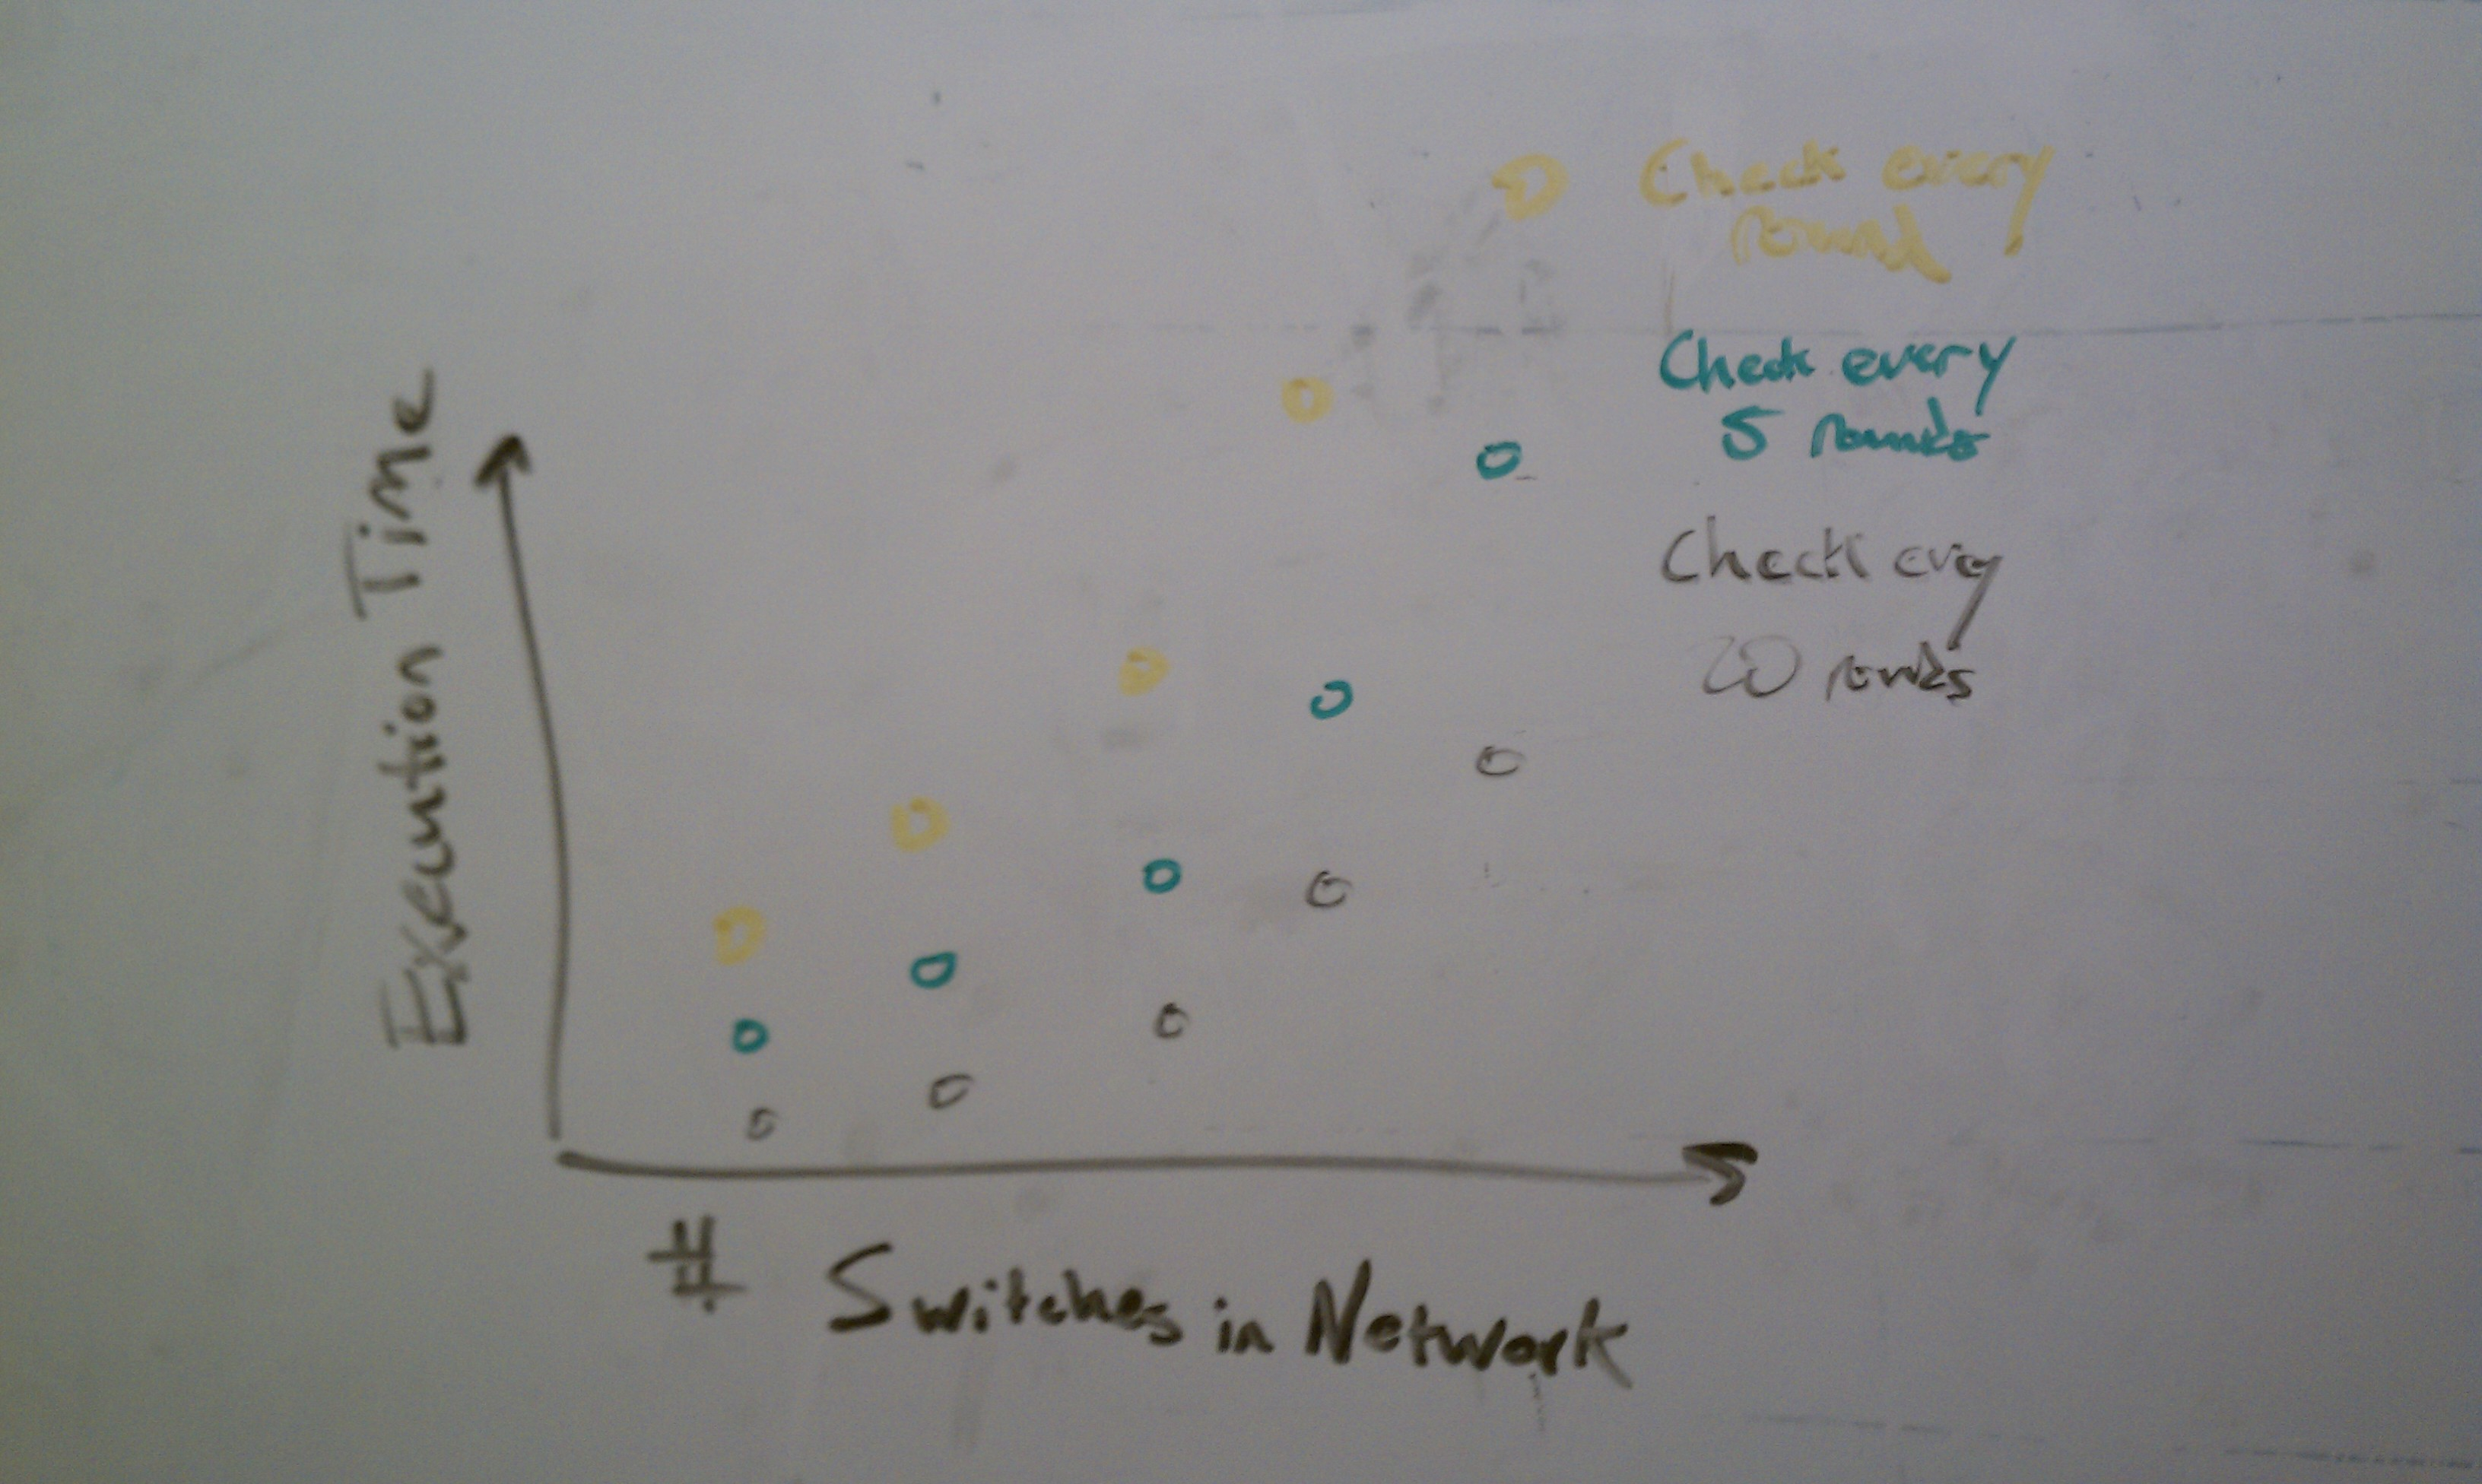
\includegraphics[width=3in]{../graphs/mock_overhead_graph.jpg}
    \caption[]{\label{fig:loop} Our lovely graph showing that execution time
    is not too bad\vspace{-10pt}} 
\end{figure}

Two orthogonal ways to ameliorate the overhead. First, you could intellegintly choose
when to run Anteater, so that you don't have to run it for every possible
configuration, while still getting good coverage of the
configuration space. Second, you could make Anteater faster, perhaps by only
getting `best-effort` exploration of the invariant checks rather than
full-blown proofs that the invariant holds. Also, Brighten mentioned that the
current version of Anteater runs significantly faster.
